\documentclass[12pt,letterpaper]{article}
\usepackage{fullpage}
\usepackage[top=2cm, bottom=4.5cm, left=2.5cm, right=2.5cm]{geometry}
\usepackage{amsmath,amsthm,amsfonts,amssymb,amscd}
\usepackage{lastpage}
\usepackage{enumerate}
\usepackage{fancyhdr}
\usepackage{mathrsfs}
\usepackage{xcolor}
\usepackage{graphicx}
\usepackage{listings}
\usepackage{hyperref}
\usepackage[section]{minted}
\usepackage{hyperref}
\usepackage{multirow}
\usepackage{caption}
\usepackage{subcaption}
\definecolor{mintedbackground}{rgb}{0.95,0.95,0.95}

\hypersetup{%
  colorlinks=true,
  linkcolor=blue,
  linkbordercolor={0 0 1}
}
 
\renewcommand\lstlistingname{method}
\renewcommand\lstlistlistingname{Algorithms}
\def\lstlistingautorefname{Alg.}

\colorlet{mygreen}{green!60!blue}

\newmintedfile[cppcode]{cpp}{
bgcolor=mintedbackground,
fontfamily=tt,
linenos=true,
numberblanklines=true,
numbersep=5pt,
gobble=0,
frame=leftline,
framerule=0.4pt,
framesep=2mm,
funcnamehighlighting=true,
tabsize=1,
obeytabs=false,
mathescape=false
samepage=true, %with this setting you can force the list to appear on the same page
showspaces=false,
showtabs =false,
texcl=false,
fontsize=\small,
breaklines
}

\setlength{\parindent}{0.0in}
\setlength{\parskip}{0.05in}

% Edit these as appropriate
\newcommand\course{EC6301}
\newcommand\name{Numerical Opimization}
\newcommand\hwnumber{3}                  % <-- homework number
\newcommand\NetIDa{20211046}           % <-- NetID of person #1
\newcommand\NetIDb{Hyeonjang An}           % <-- NetID of person #2 (Comment this line out for problem sets)
\newcommand\github{\url{https://github.com/hyeonjang/numerical-optimization}}

\pagestyle{fancyplain}
\headheight 35pt
\lhead{\github\\\NetIDa\\\NetIDb}                 % <-- Comment this line out for problem sets (make sure you are person #1)
\chead{\textbf{\Large Homework \hwnumber}}
\rhead{\course \\ \name \\ \today}
\lfoot{}
\cfoot{}
\rfoot{\small\thepage}
\headsep 1.5em

\begin{document}

\section*{Problem}

\begin{enumerate}
  \item Implement the Nelder-Mead method and the Powell's method to find the minimum of
  \begin{enumerate}
    \item $f(x, y)=(x+2y)^2 + (2x+y)^2$
    \item $(x, y)=50*(y-x^2)^2 + (1-x)^2$
    \item $f(x, y)=(1.5-x+xy)^2 + (2.25-x+xy^2)^2 + (2.625 - x+ xy^3)^2$
  \end{enumerate}
  \item Use your own termination criterion. Compare and discuss their performances. 
  If possible, show how the best point is moving on the contour plot of f(x, y)
\end{enumerate}

\section*{Implementation - methods}

\begin{enumerate}
\item Computation result: convergence points
\\ In the case of the first function, the results are the approximation of the value zero.
\\ In the case of the second function, Powell's method is sometimes stucked to local minima.
[0.510332, 0.263043] is the failure case to find optimization points.
\begin{center}
  \begin{tabular}{| c | c | c |} \hline
      \multirow{2}{*}{function $f(x, y)$}   & \multicolumn{2}{c|}{Convergence Points$(x, y)$} \\ \cline{2-3}
                                            & Nelder-Mead & Powell's  \\ \hline
      (a)                                   & [1.17932e-07, -1.85511e-07] & [-7.20495e-23, 5.73423e-23] \\ 
      (b)                                   & [1, 1] & [0.510332, 0.264043] / [0.99972, 0.999437]\\ 
      (c)                                   & [3, 0.5]  & [2.99989, 0.499973] \\
      \hline
  \end{tabular}
\end{center}
\item Implementation
  \\ initial points are randomly given. 
  \begin{enumerate}
    % ##############################################################
    % Nelder-Mead
    % ##############################################################
    \item \textbf{Nelder-Mead method}
    \\ Three control parameters are set as $\alpha=1$, $\beta=2$, $\gamma=0.5$
    \\ The maximum iteration is 10000.
    \\ The termination condition is the "magnitude of gradient".
    \cppcode[]{../../code/multi/nelder_mead.hpp}

    \newpage

    % ##############################################################
    % Powell's
    % ##############################################################
    \item \textbf{Powell's method}
    \\ For univarite searching, I used the golden section search method.
    \\ The maximum iteration is 10000 as same as Nelder-Mead method.
    \\ When using the termination criterion as the "magnitude of gradient", 
    it occurs to be stucked in local minima.
    So the termination condition is changed to "consecutive relative difference". 
    However this does not largely affect to the performance.
    \cppcode[]{../../code/multi/powells.hpp}

\end{enumerate}

\newpage

\section*{Implementation - Terminatination criterion}
\item Termination criterion
\\ I have implemented all six conditions. 
Also, to calculate the gradient of functions, 
I used numerical method to derive gradient from function given point $(x, y)$
\begin{itemize}
% ##############################################################
% Termination criterion: gradient
% ##############################################################
\item Termination criterion
\cppcode[]{../../code/multivariate.h}
\item Gradient calculation
\cppcode[]{../../code/multivariate.cpp}
\end{itemize}

\section*{Performance and Plot}
\item Performace
\begin{center}
    \begin{tabular}{| c | l | c | c |} \hline
                  & \multirow{2}{*}{function $f(x, y)$}               & \multicolumn{2}{c|}{performance} \\ \cline{3-4}
                  &                                                   & Nelder-Mead & Powell's  \\ \hline
        (a) & $(x+2y)^2 + (2x+y)^2$                                   & 872972 ns   & 84036883 ns \\ 
        (b) & $50*(y-x^2)^2 + (1-x)^2$                                & 132298767 ns& 526430665 ns \\ 
        (c) & $(1.5-x+xy)^2 + (2.25-x+xy^2)^2 + (2.625 - x+ xy^3)^2$  & 214017830 ns& 336396522 ns \\
        \hline
    \end{tabular}
\end{center}
\begin{itemize}
  \item The convergence speed of Powell's method is worse than Nelder-Mead method for every given functions.
  \item It is because Powell's method has a dependency on the univarite method.
  \item Because I have given the initial points randomly, it happens not to converge. 
  The Figure 2, which shows the result of Powell's method of the second function, is the case which cannot find the global minima.
\end{itemize}

% ##############################################################
% Plotting
% ##############################################################
\newpage
\begin{figure}
  \centering
  \begin{subfigure}[b]{0.45\textwidth}
    \centering
    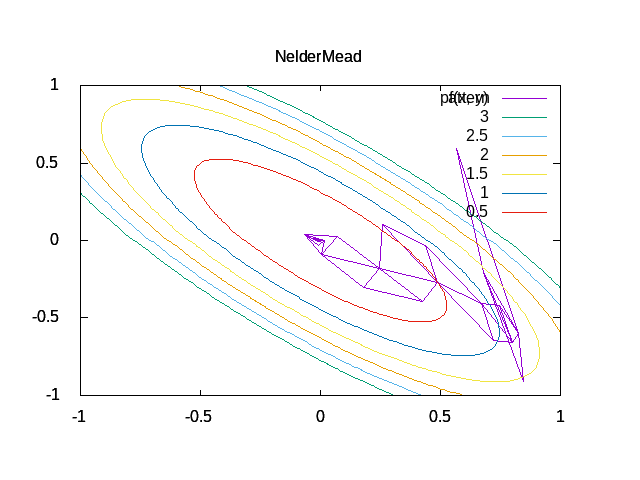
\includegraphics[width=\textwidth]{figures/NelderMead_0.png}
  \end{subfigure}
  \hfill
  \begin{subfigure}[b]{0.45\textwidth}
    \centering
    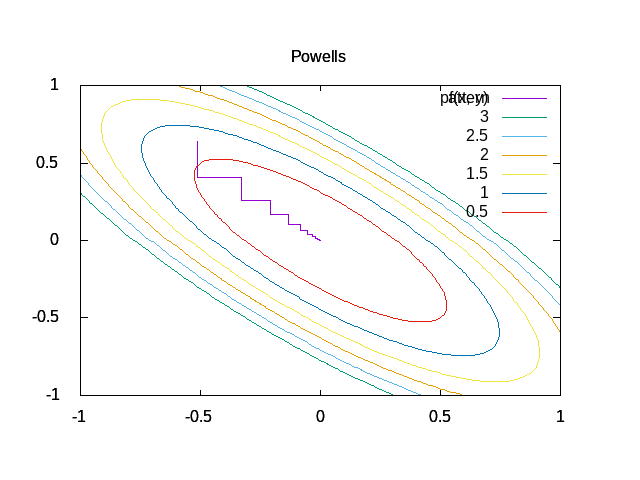
\includegraphics[width=\textwidth]{figures/Powells_0.png}
  \end{subfigure}
    \caption{$f(x, y)=(x+2y)^2 + (2x+y)^2$ }
\end{figure}

\begin{figure}
  \centering
  \begin{subfigure}[b]{0.4\textwidth}
    \centering
    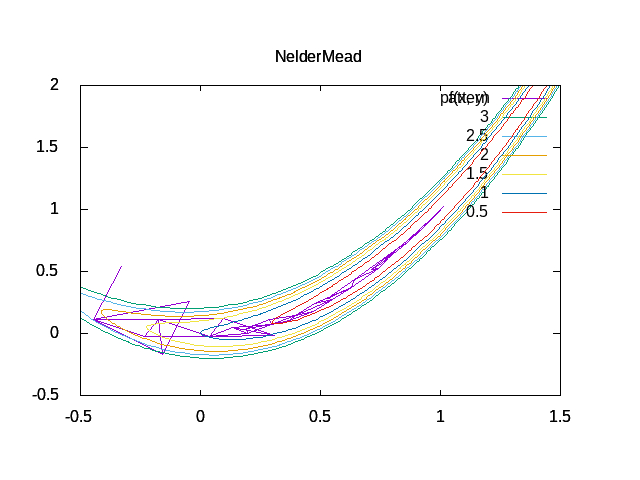
\includegraphics[width=\textwidth]{figures/NelderMead_1.png}
    \caption{Nelder-Mead}
  \end{subfigure}
  \hfill
  \begin{subfigure}[b]{0.29\textwidth}
    \centering
    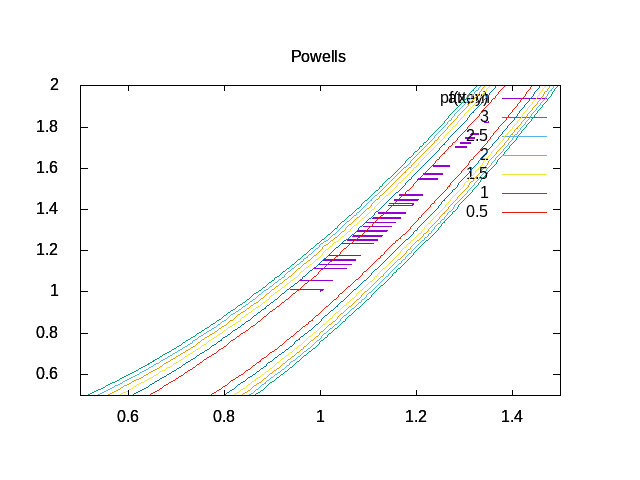
\includegraphics[width=\textwidth]{figures/Powells_1_1.png}
    \caption{Powell's: global}
  \end{subfigure}
  \begin{subfigure}[b]{0.29\textwidth}
    \centering
    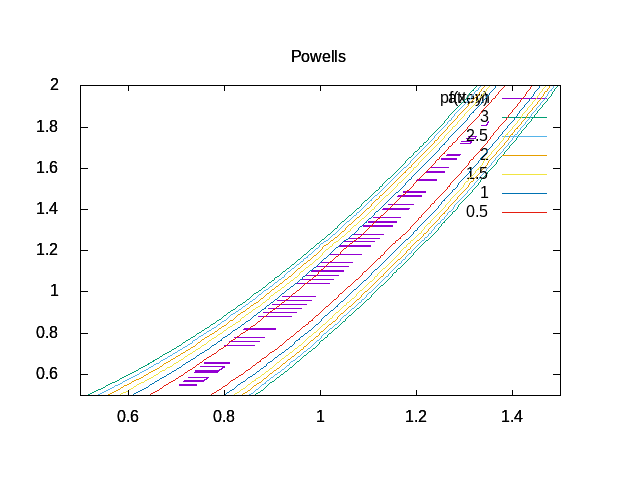
\includegraphics[width=\textwidth]{figures/Powells_1_2.png}
    \caption{Powell's: local }
  \end{subfigure}
    \caption{$f(x, y)=50*(y-x^2)^2 + (1-x)^2$}
\end{figure}

\begin{figure}
  \centering
  \begin{subfigure}[b]{0.45\textwidth}
    \centering
    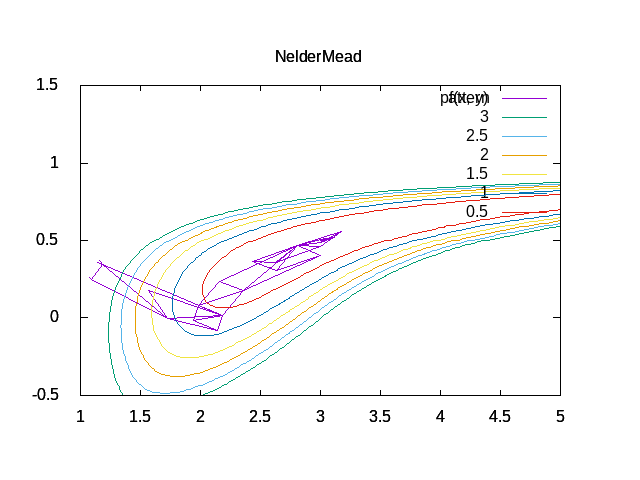
\includegraphics[width=\textwidth]{figures/NelderMead_2.png}
  \end{subfigure}
  \hfill
  \begin{subfigure}[b]{0.45\textwidth}
    \centering
    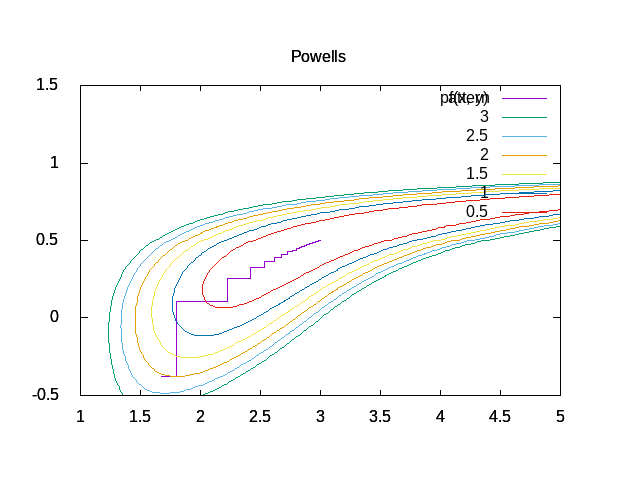
\includegraphics[width=\textwidth]{figures/Powells_2.png}
  \end{subfigure}
    \caption{ $f(x, y)=(1.5-x+xy)^2 + (2.25-x+xy^2)^2 + (2.625 - x+ xy^3)^2$ }
\end{figure}

\end{enumerate}
\end{document}